\documentclass[letterpaper]{article}

\usepackage{aaai17}
\usepackage[utf8]{inputenc}
\usepackage{times}
\usepackage{helvet}
\usepackage{color}
\usepackage{amssymb, amsmath}
\usepackage{nicefrac}
\usepackage{graphicx}
\usepackage{tikz}
\usetikzlibrary{bayesnet}

% for review
%\usepackage[displaymath, mathlines]{lineno}
%\linenumbers

\setcounter{secnumdepth}{1}

% working title
\title{Adapting Software Systems in Dynamic Environments with Probabilistic Programming}
\author{Paper \#2715 }

\DeclareMathOperator*{\argmin}{arg\,min}
\DeclareMathOperator*{\argmax}{arg\,max}
\newcommand{\mname}{PRINCESS~}

\begin{document}

\maketitle

\begin{abstract}
Modern software systems are complex, often requiring configuration of many parameters.
For long-lifespan software systems in particular, it can be difficult to select a single parameter configuration that will perform well arbitrarily far into the future.
To maintain optimal runtime performance in the presence of evolving environments, it is necessary to continually re-evaluate and re-configure a system.
In this paper, we present a probabilistic framework for online monitoring and adaptation of software.
Our framework attempts to maintain the intent of the software, as defined by a set of user-specified performance criteria, by detecting failures of intent and optimizing software parameters to restore intent.
We take a model-based approach to software optimization, and separate our focus into two distinct stages: offline learning and online adaptation.
During the offline step, we construct models of software performance with respect to software control variables.
During online adaptation, the inputs and outputs of the software are monitored and used to maintain a Bayesian model of the program's evolving environment.
If environmental changes significantly degrade system performance, an intent failure is detected, triggering re-optimization of software parameters.
Our approach makes extensive use of probabilistic programming to compose diverse software and input models.
We demonstrate the performance of this approach using two complex and dissimilar software components.
\end{abstract}

\section{Introduction}

Many software systems run on long-lifespan platforms that operate in diverse and dynamic environments.
Consider an unmanned underwater vehicle (UUV) which performs localization with a Kalman filter~\cite{murphy2012machine}.
The parameters, or \emph{control variables}, of the physical model underlying this filter are highly environment-dependent.
Weather can affect water current direction and speed. Salinity and turbidity can impact the reliability of sensor readings.
These effects are difficult to predict and correct, especially since UUVs typically must operate without a communication channel.
Even when a communication channel is available, manually adapting software or designing special-purpose adaptation routines is tedious and challenging.
A general-purpose solution to software adaptation in changing ecosystems would significantly reduce the time and effort required for maintenance, while simultaneously maintaining an optimal level of performance.

%To approach the problem of software adaptation in dynamic environments, we need : 1) a mechanism for determining when adaptation is necessary, 2) a technique for reasoning about the prevailing environment, and 3) a strategy for evaluating and enacting a particular adaptation.
%To solve the first problem, we motivate a simple notion of software \emph{intent}.
%Given a set of user-specified performance criteria, we say that a software component has violated its intent whenever these performance criteria are violated.

In this work, we present an architecture for probabilistically modeling and optimizing software components in the presence of changing input distributions.
We refer to this architecture as \mname (for Probabilistic Representation of INtent Commitments to Ensure Software Survival).
Fundamentally, this architecture aims to maintain a set of user-specified performance criteria, or the software \emph{intent}, by periodically optimizing software parameters with respect to the software's evolving usage profile.
In order to approach this problem, we need two central components: 1) a technique for reasoning about the dynamic environment, and 2) a strategy for evaluating and enacting an appropriate adaptation.

To reason about the dynamic environment, we use an \emph{input model}, which characterizes the joint distribution of environments and inputs.
In the Kalman filter example, inputs would consist of sensor readings and motor impulses, and the prevailing water current would represent an environmental factor not observable at runtime.
The input model is capable of inferring likely environmental states, in this case, the water current.
For instance, if no motor impulse is applied but the UUV's sensors indicate velocity is increasing, it is possible to infer the presence, direction, and strength of the water current.
Of course, the environment may change over time. To handle this, we present a general-purpose technique for forming \emph{posterior} input models from a stream of inputs observed at runtime.

Evaluating and enacting adaptations involves a \emph{component model}, which characterizes the distribution of component performance conditioned on input, environment, and control variables, or software parameters.
In the case of a Kalman filter, model parameters represent control variables, as these parameters may need to be tuned to achieve optimal performance in different settings. A component model for this domain could model the discrepancy between predicted and measured states, conditioned on the water current, sensor readings, motor impulses, and model parameters.
We show how the input model and component model can be coupled to optimize control variables with respect to the current environment. 
The models we consider are all implemented in the Figaro probabilistic programming language~\cite{pfeffer2010practical}.
This simplifies the composition of distinct component and input models, and facilitates the re-use of inference and optimization implementations across dissimilar software components.

Our work has three primary contributions. First, the performance-centric notion of software \emph{intent} motivated in this paper leads to a novel formulation of the software adaptation problem as optimization under uncertainty.
Second, we present a general-purpose mechanism for updating input models at runtime in order to track changes in latent environment characteristics.
Finally, the use of probabilistic programming to represent component and input models provides a flexible and extensible method for modeling systems.
We demonstrate this approach to be effective in adapting parameters for the task of state space estimation with Kalman filters and query processing with the PostgreSQL database.

\section{Related Work}

There has been a wealth of research into optimizing software configuration in \emph{offline} settings.
Typically, software optimization is formulated in a \emph{model-based} manner.
Rather than evaluating a function at all points under consideration, a model is fit to a smaller number of function evaluations, and this model is used in place of the actual function when evaluating the optimization objective.
This can lead to significant improvements in runtime when the software under study is slow to evaluate.
One popular model of software performance, known as the DACE model, uses Gaussian process regression \cite{sacks1989design}.
\citeauthor{jones1998efficient}~(\citeyear{jones1998efficient}) used the DACE model to formulate the EGO algorithm, a strategy for quickly optimizing functions which are slow to evaluate (such as complex software components).
The EGO algorithm iteratively evaluates a function of interest at a set of candidate parameters assignments and fits a Gaussian process regression model to the resulting response surface.
The Sequential Parameter Optimization algorithm of \citeauthor{bartz2005sequential}~(\citeyear{bartz2005sequential}) uses a similar ``evaluate, model, repeat'' pipeline for optimizing software parameters.
ParamILS \cite{hutter2009paramils} has been shown to be particularly effective at optimizing large spaces of software parameters using local search.
Advances in the field of software optimization are complementary to our goals, though to our knowledge PRINCESS is the first technique for optimizing software parameters in dynamic environments.

Some research into software adaptation focuses on developing software architectures that monitor and respond to degradations in system performance.
The Rainbow architecture \cite{garlan2004rainbow} employs an association between a set of performance constraints and a set of pre-specified adaptations, and triggers adaptations when a performance constraint is not met.
By contrast, our framework does not assume that adaptation strategies are pre-specified. Instead, it is the responsibility of the platform to identify an appropriate adaptation.
\citeauthor{morin2009models}~(\citeyear{morin2009models}) present a system architecture which selects an implementation for an 
abstract component at runtime using a known environmental context.
In the problem setting we consider, the environmental context is not observable at runtime and must be inferred from system usage.
In addition, instead of considering a finite, discrete system configuration space, the configuration space we consider could be infinite, 
possibly consisting of real-valued parameters.

\begin{figure*}[h!]
\centering
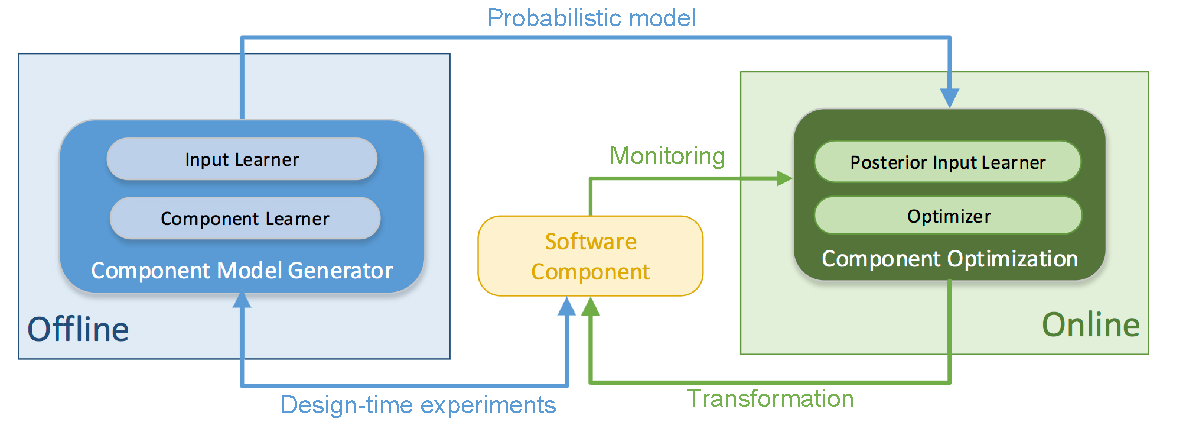
\includegraphics[width=\linewidth]{figures/architecture-overview.pdf}
\caption{System Architecture}
\label{fig:architecture-overview}
\end{figure*}

There are many self-adaptive machine learning algorithms.
For instance, adaptive versions of the Kalman filter~\cite{rutan1991adaptive,oussalah2001adaptive,wang2010adaptive} 
are able to adjust linear model coefficients or noise matrices as new observations are received.
Algorithms exist for adaptive real-time Gaussian process modeling~\cite{nguyen2009local}, support vector machine regression~\cite{cao2003support}, and Bayesian network structure learning~\cite{castillo2009adaptive}.
However, each of these algorithms is designed for adaptation of a specific, special-purpose software component.
Our work uses concepts from self-adaptive machine learning algorithms to adapt black-box software components for which no domain-specific information is available.

\section{General Approach to Adapting Components}
\label{sec:general-approach}

PRINCESS utilizes two phases, illustrated in Figure~\ref{fig:architecture-overview}.
The \emph{offline} phase involves learning probabilistic models of components.
The \emph{online} stage applies these probabilistic models to adapt components at runtime.
During the offline phase, two probabilistic models are created: an input model and a component model.
Input models express a joint distribution $\hat{P}(E, I)$ over environments and inputs.
This input model can be specified by the component designer, or can be learned from samples of environments and inputs.

The component model $\hat{P}(M|E, I, C)$ specifies a conditional density of performance metric $M$ given environment $E$, input $I$, and control variables $C$.
This model is learned in the offline phase by sampling $E$ and $I$ from the input model, sampling representative control variables $C$, and running the component at these values to measure $M$.

During the online phase, \mname has access to the stream of real component inputs $i_1, i_2, \ldots, i_k$.
This allows us to form a posterior input model, conditioned on this input stream:
\begin{align}
\hat{P}(E, I | i_1, i_2, \ldots, i_k).
\end{align}
Crucially, this posterior input model is formed using input values alone---we allow environment to be latent at runtime.
In order to track evolving input distributions, this model must be more sensitive to recent inputs than old.
We present one approach to implementing locally sensitive input models in Section~\ref{sec:implementation}. 

For each software component we consider, we assume we are given a set of performance metrics.
Each of these metrics is annotated with an upper bound.
As the true environment-input distribution diverges from the initial distribution, component performance can degrade and cause performance metrics to exceed these bounds.
We refer to this as an \emph{intent violation}.
When an intent violation occurs, an adaptation process is employed to identify the best performing control variables for the prevailing environment-input distribution.

Our method performs this adaptation using an objective function defined in terms of the input model and component model.
Suppose $cg$ represents the set of possible choices for control variable values.
The optimization problem is to find the control variable values $c^*$ such that 
\begin{align}
	c^* &= \argmin_{c \in cg} E[M|C=c] \\
		&= \int_m \int_{e, i} m \hat{P}(e, i) \hat{P}(m | e, i, c)~di~de~dm
	\label{eq:marginal-map}
\end{align}

This optimization problem (structured as in Figure~\ref{fig:optimization-model}) can be solved using marginal maximum a posteriori (marginal MAP) estimation.
To optimize multiple intent metrics, we first standardize conditional expectations to have mean zero and unit variance.
The variance $\sigma_i$ and mean $\mu_i$ for metric $i$ is estimated from the training sample.
The objective becomes a weighted sum of these standardized values, where the weights $w_i$ are designer-selected.
\begin{align}
	c^* &= \argmin_{c \in \Omega(C)} \sum_{i \in 1:|M|} w_i \frac{E[M_i|C=c] - \mu_i}{\sigma_i}
\end{align}
This standardization allows designers to specify relative weights without the need to worry about the magnitude and variability of performance metrics.

\begin{figure}[t]
	\centering
	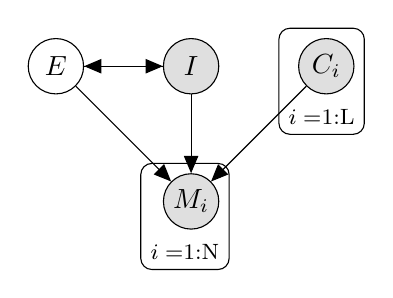
\begin{tikzpicture}
            \node[latent] (env) {$E$} ; %
            \node[obs, right=of env] (input) {$I$} ; %
            \node[obs, right=of input] (control) {$C_i$} ; %
            \node[obs, below=of input] (metric) {$M_i$} ;%
			
			\plate {metricplate} { (metric) } {$i=$1:N}; %
            \plate {controlplate} { (control) } {$i=$1:L}; %
			
            \edge {env,input,control} {metric}; %
            \edge {input} {env}; %
            \edge {env} {input}; %
	\end{tikzpicture}
	\caption{Structure of the optimization model.
	Environments and inputs are modeled jointly in an undirected manner using the input model $\hat{P}(I, E)$.
	Each component can have an arbitrary number of metrics $M_1, \ldots, M_N$.
	These metrics are affected by $I$, $E$, and all $L$ control variables $C_1, \ldots, C_L$.
	Unshaded nodes are not observable at runtime.}
	\label{fig:optimization-model}
\end{figure}

%\begin{table*}
%\centering
%\begin{tabular}{|p{1.5cm}|p{8cm}|p{8cm}|}
%\hline
%Name & Description &  Kalman Filter Implementation \\
%\hline
%I & Input & Current state, motor impulse, and sensor readings \\
%\hline
%E & Environment &  Water current \\
%\hline
%C & Control & Model parameters, including coefficients and noise terms\\
%\hline
%O & Output & Posterior state, covariance \\
%\hline
%M & Performance Metric & Covariance error volume, measurement residual \\
%\hline
%Component model & Probabilistic model of the component metrics: $P(M|E, I, C)$ & Gaussian process \\
%\hline
%Input model & Joint probability distribution of environments and inputs $P(E, I)$ & Kernel density estimator \\
%\hline
%Control prior & Prior distribution on component control values: $P(C)$ & Product of independent uniform distributions \\
%\hline
%\end{tabular}
%\caption{Modeling Types}
%\label{fig:modleing-types}
%\end{table*}


\section{Implementation}
\label{sec:implementation}

Our general framework is applicable to arbitrary input and component model implementations.
In this section, we outline the models used for our experiments.

\subsection{Input Model}

\begin{figure}[t]
	\centering
	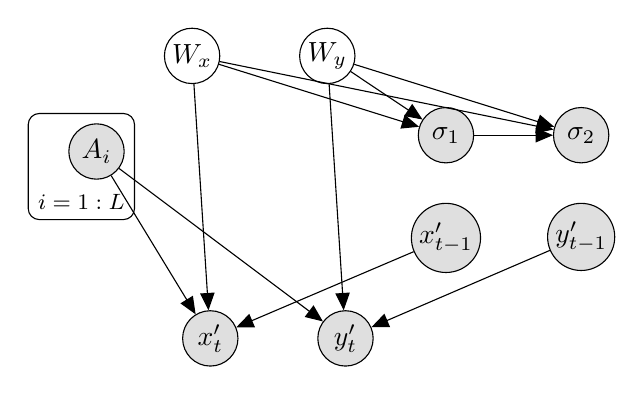
\begin{tikzpicture}
		\node[latent] (waterx) {$W_x$};
		\node[latent, right=of waterx] (watery) {$W_y$};
		\node[obs, below right=0.5cm and 1cm of watery] (covardiag) {$\sigma_1$};
		\node[obs, right=of covardiag] (covaroffdiag) {$\sigma_2$};

		\node[obs, below left=of waterx](act){$A_i$};
		\plate{actplate}{(act)}{$i=1:L$};

		\node[obs, below=0.5cm of covardiag] (s0x) {$x_{t-1}'$};
		\node[obs, below=0.5cm of covaroffdiag] (s0y) {$y_{t-1}'$};

		\node[obs, below left=of s0x] (s1y) {$y_t'$};			
		\node[obs, left=of s1y] (s1x) {$x_t'$};

		\edge {waterx, watery} {covardiag};
		\edge {waterx, watery, covardiag} {covaroffdiag};
		\edge {waterx, act, s0x} {s1x};
		\edge {watery, act, s0y} {s1y};

	\end{tikzpicture}
	\caption{Input model structure used for the Kalman filter component. The environment consists of $x$-direction water current, $W_x$, and $y$-direction water current, $W_y$, both of which are latent at runtime. The $x$- and $y$-direction velocities, $x_t'$ and $y_t'$, are dependent on the starting velocities $x_{t-1}'$, $y_{t-1}'$, actuators/motor inputs $A_i$, and the water current.}
	\label{fig:kalman-filter-input-model}
\end{figure}

The input models we consider in our applications are Bayesian networks, with structure specified by background knowledge and parameters estimated from data.
The structure of the network used for the Kalman filter domain is shown in Figure~\ref{fig:kalman-filter-input-model}.
At runtime, PRINCESS has access to a stream of time-indexed component inputs $i_{N+1}, i_{N+2}, \ldots, i_{N+K}$, which supplement the $N$ environment-input instances used to estimate the \emph{prior} parameters.
In order to estimate the posterior parameters from this input stream, we use an incremental expectation maximization (EM) approach~\cite{neal1998view}.
Unlike batch EM approaches, each step of the incremental EM algorithm operates on a single data instance.
We initialize $\theta_0^I$ and $\theta_0^E$ to be the maximum-likelihood parameter estimates on the initial sample of $N$ input and environment variables, respectively. Then, for each input $i_t$ observed at time $t$,
\begin{align}
s_t = \int_e P(e | i_t, \theta_0^I, \theta_{t-1}^E) S(e) de 
\label{eq:suff-stats-integral} \\ 
\theta^E_t = \frac{\sum_{j=0}^t \exp(-\lambda (t - j)) s_j}{\sum_{j=0}^t \exp(-\lambda (t - j))}.
\end{align}

Here, $S(e)$ represents the sufficient statistics of the data case $e$. 
The expected sufficient statistics $s_t$ are obtained by conditioning on the current input observation, $i_t$, and the current input and environment parameters $\theta_0^I$ and $\theta_{t-1}^E$.
Then, a smoothing operation is applied across the stream of sufficient statistics $s_0, s_1, s_2, \ldots, s_t$.
This smoothing step uses an exponential decay term which gives preference to recent observations, allowing the online EM algorithm to track changes in the parameter $\theta^E_t$.
The $\lambda$ parameter is the exponential decay rate, and controls how strongly the parameter estimate is biased towards recent samples.
$\lambda$ should be set in accordance with designer beliefs about the rate of state change in the environment. In our applications, environment evolves over the course of roughly 100 time units.
We set $\lambda=0.1$, such that observations made 100 time units in the past have effectively no weight.
For efficiency, we employ a third parameter, $\tau$, and discard any $s_j$ such that $\exp(-\lambda (t - j)) < \tau$. In practice, we set $\tau$ to be close to the level of machine precision, at which point $s_j$ would cease to have any effect.
We approximate the integral over environment assignments in equation~\ref{eq:suff-stats-integral} using Figaro's importance sampling algorithm.
As such, the posterior update procedure is agnostic to the form of the input model.

\subsection{Component Model}

\begin{figure}
	\centering
	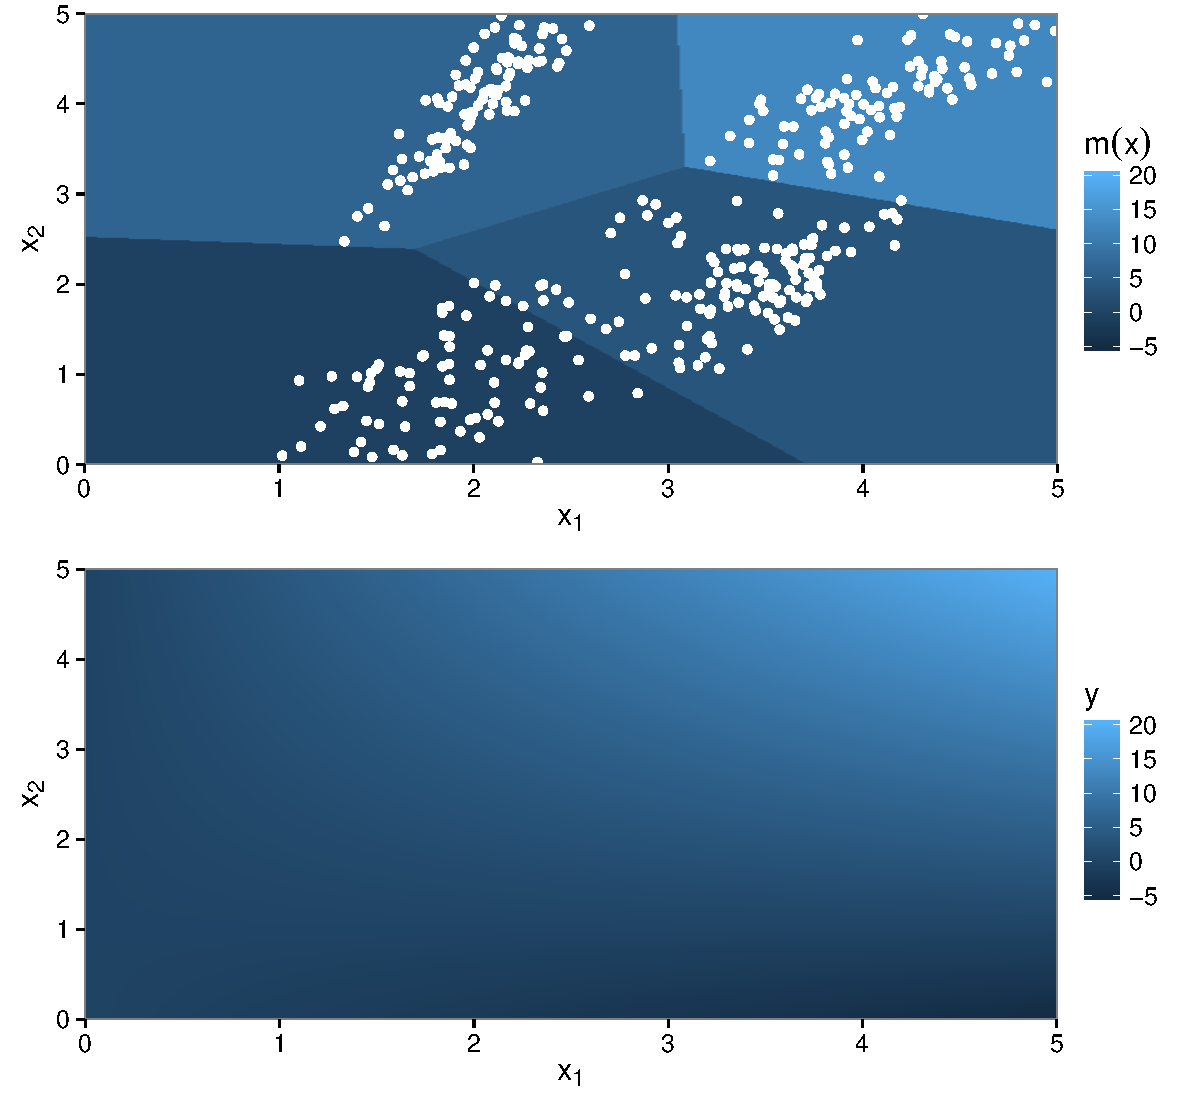
\includegraphics[width=\linewidth]{figures/mean-function-example.pdf}
	\caption{An example of the cluster-based mean function with $k=4$. The input distribution, $P(x_1, x_2)$, is multi-modal. The true response $y$ is distributed as $\mathcal{N}(x_1 x_2 - x_1, 1)$.
	The prior mean $m(x)$ is constant within sub-regions defined by the clustering (top figure). This mean function is fairly effective at capturing higher-level properties of the true response surface (bottom figure).}
	\label{fig:mean-function-example}
\end{figure}

For our experiments, we use Gaussian process regression~\cite{rasmussen2004gaussian} to perform component modeling.
A Gaussian process is specified by a \emph{mean} function $m(x)$ and a \emph{covariance} function $k(x, x')$.
Intuitively, the mean function specifies a prior belief on the response at input $x$, and the covariance function guides construction of a posterior response estimate in terms of the similarity to observed inputs.
To specify the mean function, we cluster the training inputs $x_1, \ldots, x_N$ into $k$ components, where $k$ is selected according to the Bayesian information criterion (BIC) with respect to the Gaussian process likelihood.
For a novel input $x$, we set $m(x)$ to be the mean response value in the cluster which has its center closest to $x$. An illustration of this mean function is shown in Figure~\ref{fig:mean-function-example}.
We used a squared exponential covariance:
\begin{align}
k(x, x') = \exp{\left( \nicefrac{\left| x - x' \right|^2}{\sigma^2} \right)}
\end{align}
and optimized the bandwidth parameter $\sigma$ so as to maximize the Gaussian process likelihood.
This model is similar to that considered by \citeauthor{sacks1989design}~(\citeyear{sacks1989design}).

\subsection{Optimization}

To solve the marginal MAP problem presented in equation~\ref{eq:marginal-map}, we used the CMA-ES algorithm~\cite{hansen2003reducing}.
In particular, we developed an interface which facilitates marginal MAP optimization of an arbitrary input model and component model, implemented in Figaro.
We use Figaro's importance sampling to evaluate the objective function, integrating over the support of the input model.
This approximates the quantity shown in equation~\ref{eq:marginal-map} for a \emph{given} assignment to control variables.
Since the form of the input model and component model is unrestricted, we cannot guarantee that the optimization objective is convex.
CMA-ES is suitable for non-convex, non-smooth, and poorly behaved objective functions, so it is an appropriate choice for our stochastic, non-convex objective.


\section{Applications}

To demonstrate the efficacy of PRINCESS, we created two scenarios in which software components operate in the presence of a dynamic environment.
We ran PRINCESS side-by-side with a non-adaptive baseline configuration to determine whether and by how much PRINCESS improves system performance.

\subsection{State Space Estimation}

Unmanned vehicles contain many software components that must operate and adapt without human intervention.
Unmanned underwater vehicles (UUVs) in particular must operate in complete isolation due to lack of a reliable communication channel.
Submerged UUVs do not have access to GPS readings.
To perform localization, UUVs are instrumented with sensors that can measure velocity.
UUVs have access to reliable GPS-based position information when they surface.
Once submerged, they must track their position using a state space model such as a Kalman filter~\cite{murphy2012machine}.
A Kalman filter estimates a \emph{posterior} state (after making observations) in two stages.
First, a state prediction is made using a linear state transition model taking the form:

\begin{align}
\mathbf{F} &= \begin{pmatrix}
1 & 0 & \delta & 0 \\
0 & 1 & 0 & \delta \\
0 & 0 & 1 & 0 \\
0 & 0 & 0 & 1
\end{pmatrix} \\
\mathbf{B} &= \begin{pmatrix}
0 & 0 & 0.5 m_1\delta^2 & 0 \\
0 & 0 & 0 & 0.5 m_2 \delta^2 \\
0 & 0 & m_3 \delta & 0 \\
0 & 0 & 0 & m_4 \delta
\end{pmatrix} \\
\mathbf{Q} &= \begin{pmatrix}
p_1 & 0 & 0 & 0 \\
0 & p_2 & 0 & 0 \\
0 & 0 & p_3 & 0 \\
0 & 0 & 0 & p_4
\end{pmatrix} \\
\begin{pmatrix}
\hat{x}_t \\
\hat{y}_t \\
\hat{x}'_t \\
\hat{y}'_t
\end{pmatrix} &= 
\mathbf{F}
\begin{pmatrix}
x_{t-1} \\
y_{t-1} \\
x'_{t-1} \\
y'_{t-1}
\end{pmatrix}
+ 
\mathbf{B}
\begin{pmatrix}
0 \\
0 \\
a_x \\
a_y
\end{pmatrix} \\
\mathbf{P}_{k|k-1} &= \mathbf{F} \mathbf{P}_{k-1|k-1} \mathbf{F}^T + \mathbf{Q}
\end{align}
Here, $\delta$ is the length of time between sensor readings. $\mathbf{F}$ is a standard linear model of motion.
Terms $a_x$ and $a_y$ represent current acceleration in $x$ and $y$ directions, respectively.
These would be derived from motor inputs and fluid dynamics.
The $m_1$, $m_2$, $m_3$, and $m_4$ terms are control variables which can specify influence from external forces such as water currents.
The $p_1$, $p_2$, $p_3$, and $p_4$ terms are control variables which quantify the precision of the linear model.
After making the state prediction $\left< \hat{x}_t, \hat{y}_t, \hat{x}'_t, \hat{y}'_t \right>$, 
the second stage of the Kalman filter update incorporates a vector of velocity readings $\left< z_x, z_y \right>$.

\begin{align}
\mathbf{R} &= \begin{pmatrix}
s_1 & 0 \\
0 & s_2
\end{pmatrix} \\
\vec{r} &= \vec{z} - \mathbf{H}
\begin{pmatrix}
z_x \\
z_y
\end{pmatrix}
-
\begin{pmatrix}
0 & 0 & 1 & 0 \\
0 & 0 & 0 & 1
\end{pmatrix}
\begin{pmatrix}
\hat{x}_t \\
\hat{y}_t \\
\hat{x}'_t \\
\hat{y}'_t
\end{pmatrix} \\
\mathbf{S} &= \mathbf{H} \mathbf{P}_{k|k-1} \mathbf{H}^T + \mathbf{R} \\
\mathbf{K} &= \mathbf{P}_{k|k-1} \mathbf{H}^T S^{-1} \\
\begin{pmatrix}
x_{t} \\
y_{t} \\
x'_{t} \\
y'_{t}
\end{pmatrix} &= 
\begin{pmatrix}
x_{t-1} \\
y_{t-1} \\
x'_{t-1} \\
y'_{t-1}
\end{pmatrix} + \mathbf{K} \vec{r} \\
\mathbf{P}_{k-1|k-1} &= (I - \mathbf{K} \mathbf{H}) \mathbf{P}_{k|k-1}
\end{align}

The $s_1$ and $s_2$ terms are control variables which quantify the precision of the velocity readings.
It may be difficult to select a single assignment to $m$, $p$, and $s$ that is consistently accurate.
Shifts in water currents could invalidate assignments to $m_1, \ldots, m_4$ and $p_1, \ldots, p_4$.
If sensor reliability depends on oceanographic factors, no single assignment to $s_1$ and $s_2$ would be appropriate.

The scenario we consider here is one with two latent environment features: $x$- and $y$-direction water currents.
The input features $I$ consist of an initial state $\left< x_{t-1}, y_{t-1}, x'_{t-1}, y'_{t-1} \right>$, an initial covariance $\mathbf{P}_{t-1|t-1}$, and an observation $\vec{z}$.
The Kalman filter performance metric is $| \vec{r} |$, the magnitude of the prediction-observation discrepancy.
When $| \vec{r} |$ exceeds 5, an intent violation is triggered.

\begin{figure}
	\centering
	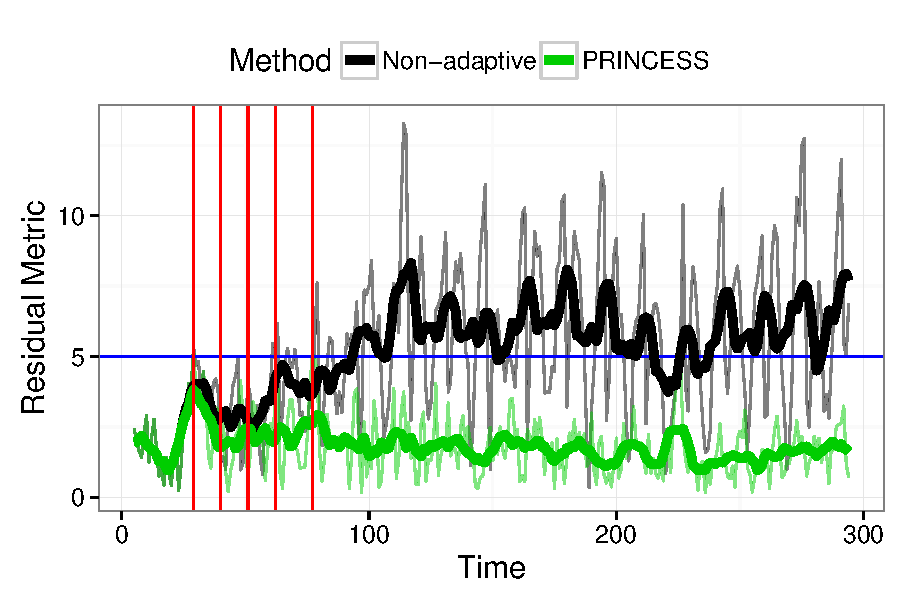
\includegraphics[width=\linewidth]{figures/kf-optimization-example.pdf}
	\caption{One simulation from the state space estimation problem, showing the performance (in terms of the measurement residual) of PRINCESS and the static baseline. 
	Bold lines are 5-step moving averages, and thin lines track individual values.
	The horizontal blue line indicates the point of intent violation.
	Vertical red lines indicate times at which optimization was performed, consistent with the times of intent violation.
	PRINCESS is able to maintain system performance in the presence of environmental changes, while the baseline does no adaptation.}
	\label{fig:state-space-estimation-example}
\end{figure}

\begin{table}[t]
\centering
\begin{tabular}{ll}
  \hline
Method & AUC \\ 
  \hline
Non-adaptive & 1558.49 (27.88) \\ 
  PRINCESS & \textbf{582.07 (129.1)} \\ 
   \hline
\end{tabular}
\caption{
Performance of PRINCESS and the non-adaptive baseline on the state space estimation task.
The mean area under the curve of measurement residuals (as shown in Figure~\ref{fig:state-space-estimation-example}) across all 50 simulations is shown, with one standard deviation shown in parenthesis.}
\label{fig:state-space-estimation-results}
\end{table}

We simulated 50 trajectories of 300 consecutive inputs to the Kalman filter, varying the UUV acceleration.
The system is initialized with control variables appropriate in the absence of a water current (all $m_i$ = 1).
We simulated gradual increase in water current until $t=100$, at which point optimal control variables are $m_1 = 2$, $m_2 = 0.5$, $m_3 = 2$, and  $m_4 = 0.5$.
Two system configurations are considered.
The first is a static baseline which continues to use the increasingly inappropriate control variables as the environment changes.
The second uses PRINCESS to monitor system performance, in this case the filter's measurement residual.
As shown in Table~\ref{fig:state-space-estimation-results}, we found that PRINCESS was able to significantly improve the performance over the baseline configuration. Figure~\ref{fig:state-space-estimation-example} shows a representative trajectory. In this case, PRINCESS detected 5 intent violations, all occurring in the interval $t \in [0, 100]$, consistent with the interval in which environment is regularly changing.

\subsection{Query Processing}

Consider a data warehousing environment in which a database server experiences periodic shifts in query workload.
In this case, the latent query workload specifies which queries are more likely than others, and represents an environment in our framework.
An individual query sampled from the query workload takes the role of a component input.
Query runtime is a natural performance characteristic, but is highly variable.
In this case, instead of monitoring intent at the level of individual inputs, we trigger an intent violation whenever a 10-step moving average of runtime exceeds 500 milliseconds.
The task of PRINCESS is to minimize runtime with respect to the prevailing query workload.

Several factors of the database configuration affect runtime, including the extent of indexing, disk access cost estimates supplied to the database engine, and the amount of memory supplied to the database engine.
These configuration variables take the role of control variables in this scenario.
The queries we used are real, human-written queries, collected for a factorial experiment carried out on the PostgreSQL database by~\citeauthor{garant2016evaluating}~(\citeyear{garant2016evaluating}).
Each query is executed using every combination of configuration variables, yielding a dataset with ground truth performance measurements for every possible input query and control assignment.

\begin{figure}
	\centering
	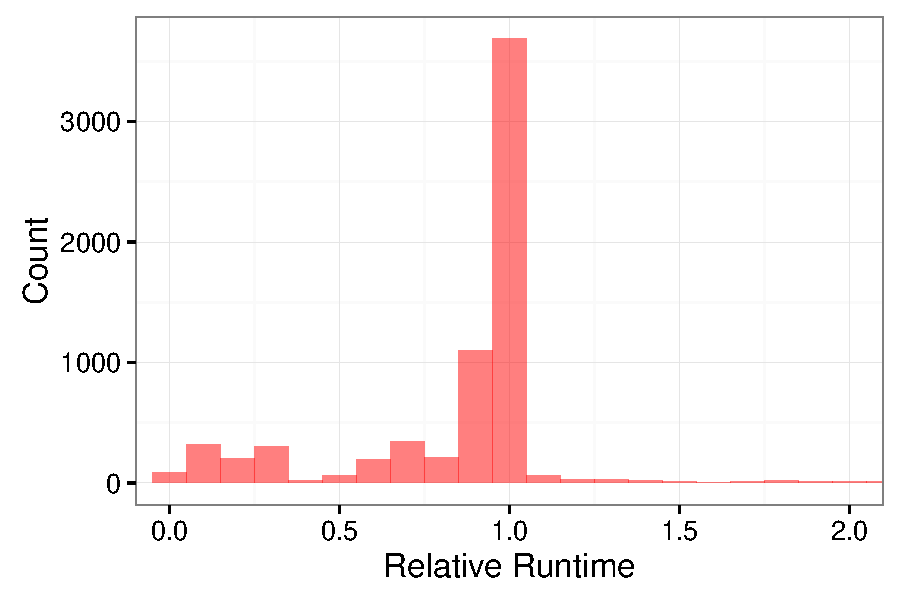
\includegraphics[width=0.9\linewidth]{figures/pg-relative-performance.pdf}
	\caption{Histogram of PRINCESS-optimized performance relative to the non-adaptive baseline on the query processing domain.
	For clarity, we omitted a long right tail from this plot, with maximum 11.05, that represented only 2\% of the overall mass.}
	\label{fig:query-processing-results}
\end{figure}

We simulated 20 batches of 300 queries.
The first 100 queries produce a relatively small number of records, and the second 200 queries produce a relatively large number of records,
consistent with a shift in the nature of the query workload.
Control variables are initialized such that low-complexity queries can be answered quickly.
We compared the trajectory of runtimes obtained by a PRINCESS-optimized system to those obtained by continuing to use the low-complexity control variables for the full batch of 300 queries.
Since runtime is highly variable, we show \emph{relative} runtimes in our results, which is the runtime of PRINCESS divided by the baseline runtime under the same input.
Figure~\ref{fig:query-processing-results} illustrates that PRINCESS is able to improve system performance on most input queries.
In particular, for 69\% of the cases, PRINCESS has found control variables that yield improved runtime. In 9\% of the instances, PRINCESS has not yet found control variables which differ from the baseline. In the remaining cases, the control variables identified by PRINCESS degrade performance.

\section{Conclusions and Future Work}

We have developed a modular probabilistic framework for dynamic program adaptation.
To our knowledge, this is the first technique to \emph{learn} software adaptation strategies in \emph{online} settings in which environmental characteristics experience change.
We have shown this technique to be advantageous in optimizing the control variables of two dissimilar software systems, achieving and maintaining significantly better performance than a non-adaptive baseline configuration.
Our use of probabilistic programming simplifies the extension of this general methodology to additional software systems.

Our work has focused on independently modeling software components.
However, across a system of interacting components, the performance of one component is likely to be causally dependent on or correlated with the performance of other components.
One promising future direction would be to explore efficient learning of dependent component models.
We are also interested in exploiting system decomposition to solve a large-scale optimization problem using a set of small-scale solutions.

\bibliography{bib}
\bibliographystyle{aaai}

\end{document}
